\documentclass[a4paper,12pt, twoside]{article}
%\documentclass[a4paper,12pt, twoside]{book}

\usepackage[papersize={210mm,297mm},tmargin=20mm,bmargin=20mm,lmargin=20mm,rmargin=20mm]{geometry}

\usepackage[utf8]{inputenc}
%https://mirror.hmc.edu/ctan/macros/latex/contrib/babel-contrib/turkish/turkish.pdf
\usepackage[english]{babel}
%\usepackage[T1]{fontenc}

\usepackage{amsmath,amssymb,mathabx}%\for eqref
\usepackage{lscape}

\usepackage{hyperref}
\hypersetup{
    colorlinks,
    citecolor=black,
    filecolor=black,
    linkcolor=blue,
    urlcolor=red}
  

%%% \usepackage{svg}
%%% https://tex.stackexchange.com/questions/122871/include-svg-images-with-the-svg-package/129854
\usepackage{graphicx}
\graphicspath{ {./figurler/} }

\usepackage[colorinlistoftodos]{todonotes}
\usepackage{fancyhdr}

\usepackage{indentfirst}
%% paragraf girintisi
\setlength{\parindent}{5ex}

%% Daha sonra yazılacak kısımları not düşmek için...
\newcommand{\YAZILACAK}{{\vspace{18pt}\bf\Large \color{red} YAZILACAK}}


\pagestyle{fancy}
\fancyhf{}
\lhead{ Kuantum Fiziği }
\chead{\thepage}
\rhead{Mesut Karakoç}
\lfoot{Akdeniz Üniversitesi}
\cfoot{}
%\rfoot{BF}

\title{Akdeniz Üniversitesi\\ Fen Fakültesi - Fizik Bölümü\\FİZ319 Kuantum Fiziği Ders Notları}

\author{\setlength{\unitlength}{6mm}
\begin{picture}(10,10)
\put(1.1,0){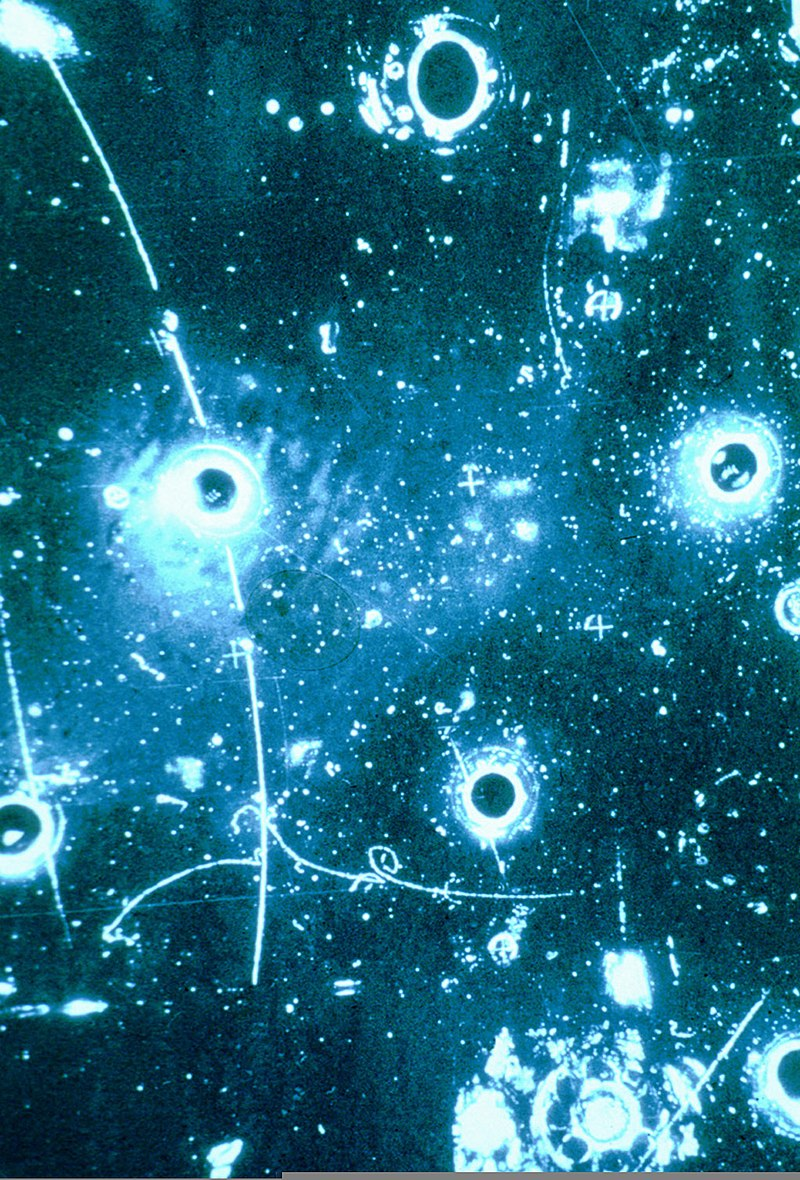
\includegraphics[width=4.5cm]{Leptonic_event_in_Gargamelle_bubble_chamber.jpg}}
\end{picture} \\ Doç. Dr. Mesut Karakoç}


\date{\today}

\begin{document}

%% Turkish babel problem
%% https://tex.stackexchange.com/questions/160385/newgeometry-doesnt-work-with-turkish-babel-package
%%\shorthandoff{=}% Make = not active any more

\maketitle

\newpage

% change name to "İçindekiler"
\renewcommand{\contentsname}{İçindekiler}
\tableofcontents{}

\listoffigures
 
\listoftables

\newpage

{
\hspace{.5\textwidth}
\begin{minipage}{.5\textwidth}
\raggedleft
If all this damned quantum jumps were really to stay, I should be
sorry I ever got involved with quantum theory.

—Erwin Schrödinger
\cite{book:Ficek}

%% Latince için
%% post iacturam quis non sapit!
%% Who is not wise after he has lost something?
%% https://quizlet.com/23756827/latin-proverbs-h-flash-cards/
\end{minipage}
}

\setcounter{section}{1} %% THIS WILL BE DELETED when all chapters merged!
\section{Dalga-Parçacık İkilemi ve Schrödinger Denklemi}

Kuantum fiziğinin doğum sürecini anlattığımız bir önceki bölümün içeriği genellikle \emph{Eski Kuantum Teorisi} olarak adlandırılır. Çünkü, gerçekleştirilen keşifleri açıklamak için  kullanılan veya ortaya konan kuralların tam olarak birbirleriyle sağlam bir bağlantısının olduğunu söylemek pek mümkün değildir. Daha iyi bir açıklama için ortaya konan ``Kuantum Mekaniği" iki defa keşfedilmiştir denebilir, ilki 1925'te matris mekaniği formalizmiyle Werner Heisenberg tarafından ve ikincisi 1926'da dalga mekaniği ile Erwin Schrödinger tarafındandır. Her ikisinin eş değer olduğu sonradan gösterilmiş olmasına rağmen Schröndinger'in yöntemi daha çok kullanılır hale gelmiştir. Çünkü dalga mekaniğinin matematiği fizikçiler arasında daha yaygındı \cite{book:Gasiorowicz}.


\subsection{Dalga-Parçacık İkilemi}
Kuantum fiziğini başlatan deneyler ve deneyleri açıklamak için geliştirilen teori ve modeller; klasik fizikte parçacık olarak bilinen (elektron, proton, nötron vb.) fiziksel varlıkların dalga özellikleri gösterdiklerini, benzeri şekilde dalga özelliği gösteren elektromanyetik dalganın parçacık (foton) özelliği gösterdiğini doğrulamıştır. 


\begin{figure}[hbtp]
\center

\includegraphics[scale=.5]{Wave-particle.png}
\caption{Işık bir dalgadır!?}
\label{fig:light_is_a_wave}
\end{figure}

Bu durumda kuantum fiziğinin sınırları içine giren herhangi bir fiziksel varlık, hem dalga hem de parçacık davranışı gösterebilmektedir. Dalga özelliği gösteriyorsa; kutuplanma, girişim ve kırınım gibi davranışlar göstermesi beklenirken, parçacık özelliği gösterdiğindeyse; klasik fizikteki gibi enerji ve momentum taşıması beklenmektedir. Belirli şartlar altında ışığın veya herhangi bir elektromanyetik dalganın enerji ve momentum taşıdıkları fotoelektrik etkisi, Compton saçılması ve karacisim ışıması deneylerinde göz1enmiştir.

Fakat her iki özelliğin de gözlenebiliyor olması öyle kolayca anlaşılamayabilir. Compton etkisi (veya saçılması) deneyiyle ışığın foton adı verilen bir parçacık gibi davrandığı doğrulanmıştır. İnsan gözüyle fotonlar tek tek seçilemese de, fotonları tek tek seçebilen ve fotoçoklayıcı \cite{book:Gasiorowicz} olarak adlandırılan cihazlar mevcuttur. 

Dirac'ın kuantum mekaniği üzerine yazdığı bir kitabında ilginç bir düşünce deneyi vardır. Belirli bir kutuplanmaya sahip ışık fotoelektrik etkide olduğu gibi elektron elde etmek için kullanılırsa, yayınlanan elektronların açısal dağılımı fotonların kutuplanmasıyla ilişkilidir. Fotoelektrik etkiye göre bir foton bir elektron koparabildiğine göre, fotonlar enerji ve momentuma ek olarak kutuplanmaya da sahiptir. Buna göre başlangıçta $I_0$ şiddetine sahip ve kutuplanmış bir ışık demetini sadece belli bir kutuplanma eksenindeki ışığın geçmesine izin veren bir kristalden geçirdiğimizi düşünelim. Eğer gelen ışığın tamamı kristalden geçecek kutuplanmaya sahipse geçen ışığın şiddeti de $I_0$ olacaktır. Eğer kutuplanma vektörü kristalin kutuplandırma ekseni ile $\theta$ açısı kadar farka sahipse, geçen ışık şiddeti $I_0 \cos^2 \theta$'a kadar olur. Bu durumu her bir foton için tek tek ele alalım. Eğer ışık demeti tamamen kristalin kutuplanma ekseni ile aynı yönde kutuplanmışsa demeti oluşturan bütün fotonların hepsi aynı yöndeki kutuplanmaya sahiptir. Fakat farklı bir polarizasyona (kutuplanmaya) sahip bir ışık demetinde ise demetin şiddeti  $\cos^2 \theta$ ile belirlenen oran kadar azalacaktır. Bunun anlamı bu oran kadar fotonun kristalden geçebilmesidir. Fakat, \emph{fotonlar bölünemezler} bu durumda bir foton kristalden ya geçer ya da geçemez. Bireysel olarak hangi fotonun geçtiğini bilmemiz mümkün değildir. Bütün söyleyebileceğimiz $N$ tane foton geldiyse, bunun $N \cos^2 \theta$ kadarının geçtiğidir. Böyle bir fotonun bu kristalden geçebilme olasılığı $\cos^2\theta$ olur.

Klasik optik fiziğine göre  bir çok foton içeren bir ışık demeti girişim ve kırınım gibi dalga özellikleri gösterecektir. Işığın dalga özelliğinin tek bir foton için de geçerli olduğunu gösteren bazı deneyler gerçekleştirilmiştir. Bunlardan birisi de G. I. Taylor tarafından 1909 yılında yapılmıştır. Bu deneyde bir iğne ucu etrafında çok düşük şiddetteki (bir kerede bir fotonun geçtiği) ışığın bile kırınıma uğradığı gösterilmiştir. Bu bize ışığın dalga davranışının fotonların toplu (kollektif) bir davranışı sonucunda değil de, bireysel özelliklerinin bir sonucu olarak var olduğunu göstermiştir. Bu durumda yeni sorunlar ortaya çıkmaktadır.


\begin{figure}[hbtp]
\center
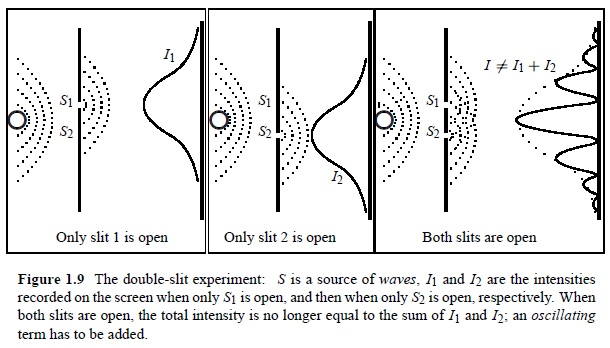
\includegraphics[scale=.8]{Double-slit_experiment_unknown_source.png}
\caption{Buraya benzeri bir başka şekil konacak!}
\label{fig:dobule_slit_experiment}
\end{figure}

Taylor'un deneyinin bir benzeri olan çift yarık deneyini düşünelim. Diğer deneydeki gibi her defasında bir foton gelsin ve Şekil \ref{fig:dobule_slit_experiment}'deki gibi yarıklardan birinden geçtikten sonra arkadaki ekranda yakalansın. Her iki yarıkta açıkken, yeterince sayıda foton geçtikten sonra klasik olarak beklendiği üzere (ışık dalga olduğundan) Şekil \ref{fig:dobule_slit_experiment}'in en solundaki gibi bir girişim deseni gözlenir. Klasik olarak bu durum çok rahat açıklanabilir. Eğer yarık 1 ve yarık 2'den geçen elektromanyetik dalgalar $\vec E_1(\vec r, t)$ ve $\vec E_2(\vec r, t)$ ile temsil edilirlerse, arkadaki ekrandaki bir $\vec r$ konumunda $t$ anında toplam dalga bu iki dalganın toplamı olacaktır. Bu klasik elektromanyetik teorinin bir parçası olan Maxwell denkleminin lineer olması dolayısıyla üst üste binme (süperposizyon) ilkesine uymasının sonucudur. Arkadaki ekranda gözlenecek olan ışığın toplam şiddeti ise,
%%
\begin{equation}
I \,\, \propto\,\, E^2 = \vec E \cdot \vec E = |\vec E_1 + \vec E_2|^2 = E_1^2 + E_2^2 + 2\vec E_1 \cdot \vec E_2
\label{eq:foton_interference}
\end{equation}
%%
denklemi ile belirlenir. Oluşan girişim deseninin matematiksel kaynağı $\vec E_1 \cdot \vec E_2$'dir. Eğer iki yarıktan sadece birisi açık olsaydı, sadece $|\vec E_1|^2$ veya $|\vec E_2|^2$ ile orantılı şiddetler gözlenebilirdi. Eğer bu şiddetleri polarizasyon deneyinde olduğu gibi olasıkla ilişkilendirirsek, sadece birinci veya ikinci yarıktan geçme olasılıkları sırasıyla $P_1(r,t)$ ve $P_2(r,t)$ olurken, her iki delik açıkken geçme olasılıkları bu iki olasılığın doğrudan toplamı olmaz.

Fotonlar bölünemez olduklarına göre ve bu davranış tek bir foton için de geçerli olduğuna göre, bu durum ancak \emph{bir fotonun kendi kendisiyle girişim} yapabileceğini varsaymakla çözülebilir. Böyle bir fotonun iki yarıktan açıkken sahip olacağı klasik elektromanyetik dalga alanı,
%%
\begin{equation}
\vec e = \vec e_1 + \vec e_2
\label{eq:single_foton_em_field}
\end{equation}
%%
şeklinde olacaktır ve Maxwell'in çizgisel klasik elektromanyetik dalga denklemlerine uygun olacaktır. Polarizasyon deneyinde olduğu gibi bu deneyde de tek bir fotonun hangi yarıktan geçtiğini bilmek mümkün değildir.


İlk keşfedildiklerinde elektronların parçacık yönüyle karşılaşılmıştır. Klasik olarak hareketlerinin yörüngesi üzerlerine etki eden manyetik ve elektrik alanlar ile belirlenebilir, kütlelidirler, enerji ve momentum taşırlar. Daha sonraları elektron kırınımı ve elektron için çift yarık deneyleriyle elektronların da dalga davranışı gösterdikleri gösterilmiştir. Elektron için gerçekleştirilen çift yarık deneyinde de, yukarıda foton için gerçekleştirdiğimiz düşünce deneyine benzer şekilde, elektronların çift yarıktan geçtikten sonra arkadaki ekranda girişim desenleri oluşturdukları gözlenmiştir. Fotonlarda girişim deseninin oluşma nedeni toplu bir davranışın değil bireysel davranışların sonucuydu, elektronların girişim deseni de aynı şekilde bireysel bir davranışın sonucudur. Foton için tanımladığımız gibi elektronun kendi kendisiyle girişimini ifade eden bir dalga fonksiyonu tanımlamak mümkündür. Böylece çift yarık deneyindeki bir elektronun dalga fonksiyonu,
%%
\begin{equation}
\psi(\vec r, t) = \psi_1(\vec r, t) + \psi_2(\vec r, t)
\label{eq:single_electron_wave}
\end{equation}
%%
olarak yazılabilir. Bu dalga fonksiyonunun elektronun girşimini izah eden çizgisel bir denkleme uyması beklenir. Böylece elektronun yarıklardan birisi açık olduğundaki dalga fonksiyonlarının toplamı, üst üste binme ilkesi gereğince, her iki yarık açık olduğundaki dalga fonksiyonunu vermelidir. Böyle bir dalga fonksiyonunu kullanan ünlü bir çizigisel denklem {\bf Schrödinger denklemi}'dir. Bu denklemde $\psi (\vec r, t)$ elektronun $\vec r$ konumunda ve $t$ anında ikinci ekranda bulunma olasılığıyla ilişkilidir. 

\subsection{Düzlem Dalgalar ve Dalga Paketleri}

Bu bölümde sıradan düzlem dalgalardan yola çıkarak elektron gibi bir parçacığın parçacık özelliklerini de içerecek olan \emph{dalga paketi} kavramını incelyeceğiz. Bu dalga paketleri parçacıkları temsil etmekle beraber, sanki gerçekten parçacık gibi davranan dalga paketleri varmış gibi düşünmek doğru değildir \cite{book:Gasiorowicz}.

Basit harmonik bir hareketi tanımlayan $k$ dalga sayısına sahip ve $+x$ yönünde ilerleyen bir dalga,
%%
\begin{equation}
\psi_k(x, t) = A_1 \cos(kx - \omega t) + A_2 \sin(kx - \omega t)
\label{eq:plane_sin_wave}
\end{equation}
%%
olarak veya,
%%
\begin{equation}
\psi_k(x, t) = A \text{e}^{i(kx - \omega t)} + B \text{e}^{-i(kx - \omega t)}
\label{eq:plane_exp_wave}
\end{equation}
%%
şeklinde yazılabilir. Dalga sayısı ve dalga boyu arasında, açısal frekans ve periyot arasında ve açısal frekans ile frekans arasında sırasıyla aşağıdaki bağıntılar vardır;
%%
\begin{equation}
k = 2\pi/\lambda, \,\,\,\, \omega = 2\pi/T,\,\,\, \text{ve}\,\,\, \omega = 2\pi\nu.
\label{eq:wave_length_number}
\end{equation}
%%
Klasik dalgalardan hatırlanacağı üzere $\omega$ ve $k$ arasındaki bağıntı, bir dalganın dağınımlı bir ortamda mı, yoksa dağınımsız bir ortamda mı ilerlediğiniz belirlemektedir. Örneğin boşlukta ilerleyen ışık (veya elektromanyetik dalga) için $\omega$ ve $k$ arasındaki bağıntı,
%%
\begin{equation}
\omega = 2\pi \nu = 2 \pi c/\lambda \text{, olduğundan }\, \omega = c k
\label{eq:w_k_relation}
\end{equation}
%%
olur. Çünkü dağınımsız ortamlarda $\omega$ ve $k$ doğru orantılıdır. Dağınımlı bir ortam da ise açısal frekans dalga sayısının ($\omega(k)$) bir fonksiyonu olarak yazılabilir. Örneğin, dağınımlı ortamda ışığın frekansı ortamın kırılım indeksine bağlı olarak $\nu = c/n\lambda$ şeklinde yazılabilir. $n$ ise genellikle $\lambda$'nın bir fonksiyonudur. Doğal olarak $\omega$ ve $k$ arasındaki doğru orantının kaybolacağı açıktır.
%%
\begin{figure}[hbtp]
\center
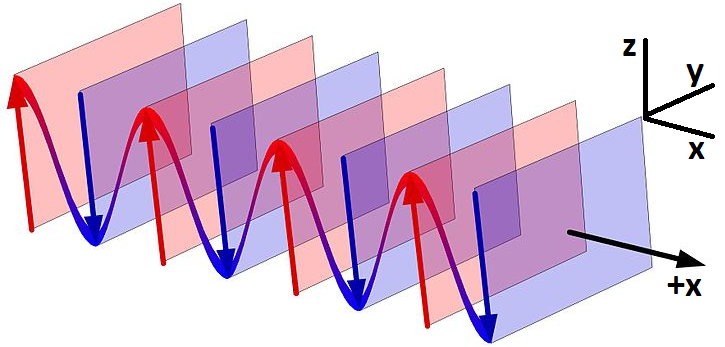
\includegraphics[scale=1.5]{Plane_Wave_Oblique_View.png}
\caption{$+x$ yönünde ilerleyen ve $y-z$ düzleminde sabit değerli olan düzlem dalganın temsili çizimi.}
\label{fig:plane_wave}
\end{figure}
%%
%%
Şimdi yukarıdaki bilgilere göre dalga paketi kavramını tanımlaya çalışalım. $\psi_k(x,t)$ $y$ ve $z$'den bağımsız olduğu için Şekil \ref{fig:plane_wave}'deki gibi bir davranışa sahip düzlem dalgadır. $\psi_k(x,t)$ ile bir kuantum davranışlı varlığın (elektron, foton v.b.) bütün sahip olabileceği $k$ değerli dalga fonksiyonlarını tanımlamak mümkündür. Çift yarık deneyinde elektron veya foton için sadece iki dalga fonksiyonunun süperpozisyonu söz konusuyken bu durumda bütün olası durumları göz önüne alabilmek için genliği $k$'ye bağlı $A(k)$ genlikli,
%%
\begin{equation}
\psi_k(x, t) = A(k) \text{e}^{i(kx - \omega t)} 
\label{eq:plane_wave_A_k}
\end{equation}
%%
bir ilerleyen düzlem dalga yazmak mümkündür. Bu düzlem dalgaların süperpozisyonu ise,
%%
\begin{equation}
\psi(x, t) \equiv \int\limits_{-\infty}^{\infty}dk\,\psi_k(x, t) = \int\limits_{-\infty}^{\infty}dk\,A(k) \text{e}^{i(kx - \omega t)} 
\label{eq:wave_packet}
\end{equation}
%%
ile elde edilir. Süperpozisyon sonucu elde edilen bu dalga fonksiyonu, \emph{dalga paketi} olarak adlandırılır. Dalga paketi $t=0$'da
%%
\begin{equation}
\psi(x, 0) = \int\limits_{-\infty}^{\infty}dk\,A(k) \text{e}^{i(kx)} 
\label{eq:wave_packet_t0_int}
\end{equation}
%%
olur. Klasik parçacıklar dalgalardan farklı olarak belirli bir konuma sahip olduklarından ve bir dalga paketi ile parçacık özelliklerini tanımlamak istediğimizden, dalga paketinin erişimi de sonlu bir dağılım olmalıdır. Bu nedenle $A(k)$,
%%
\begin{figure}[hbtp]
\center
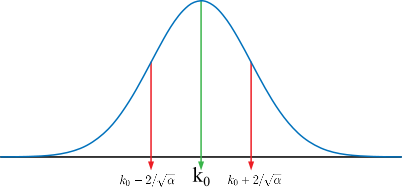
\includegraphics[scale=1.5]{Gaussian_distribution.png}
\end{figure}
%%
\begin{equation}
A(k) = \text{e}^{-\alpha (k-k_0)^2/2}
\label{eq:wave_packet_t0}
\end{equation}
%%
gibi, gausyen (gaussian) dağılım olarak adlandırılan, bir dağılım tercih edilebilir. Bu dağılımın merkezi $k_0$ civarındadır ve merkezden uzaklaşırken hızlıca değeri azalır. Daha sonra bir parçacığın momentumunun belirli bir aralıkta olma özelliğini tanımlayan bu fonksiyonun karesinin önemli olduğunu göreceğiz. Kare fonksiyonun tepe değerinden $\frac{1}{3}$ değerine $\alpha (k-k_0)^2\eqsim 1$ civarında düşer. Buna göre bu dağılımın genişliği $\Delta k \equiv = k-k_0 = 2/\sqrt{\alpha}$ olarak tanımlanabilir. $t=0$'daki dalga paketini tanımlayan integral önce $q' = k-k_0$ değişken dönüşümü yapılarak,
%%
\begin{equation}
\psi(x, 0) = \text{e}^{ik_0x} \text{e}^{x^2/2\alpha} \int\limits_{-\infty}^{\infty}dq' \, \text{e}^{-\alpha q'^2/2} = \sqrt{\frac{2\pi}{\alpha}} \text{e}^{ik_0x} \text{e}^{x^2/2\alpha}
\label{eq:wave_packet_t0}
\end{equation}
%%
şeklinde çözümlenebilir. Sabitleri göz önüne almazsak elde ettiğimiz dalga paketi sanki yeni bir dağılım fonksiyonuyla düzlem dalganın çarpımı gibi durmaktadır. Bu yeni dağılım fonksiyonu parçacığı $x=0$ civarında yerelleştirmeye çalışmaktadır. $A(k)$ dağılım fonksiyonuna benzer şekilde bu dağılım fonksiyonun genişliği ise $\Delta x \equiv  x - 0 = 2\sqrt{\alpha}$'dır. İlginç bir şekilde dalga paketinin şeklini belirleyen $\Delta k$ ve $\Delta x$ genişliklerinin çarpımı,
%%
\begin{equation}
\Delta k  \Delta x  = 4
\label{eq:del_x_k}
\end{equation}
%%
değerine sahiptir ve $\alpha$'dan bağımsızdır. Bu ilişki Fourier türü integrallerin genel bir özelliğidir.


Bir dalga paketinin $t=0$ anında sahip olabileceği formunu ve bu formun genişliğini sınırlayan bir bağıntı elde etmiş olduk. Bu dalga paketinin zamanla nasıl ilerleyeceğini ise (şimdilik) yaklaşık olarak çalışmak yeterlidir. Bu yaklaşıklıkta $k_0$ etrafında çok dar bir dağılıma sahip bir dalga paketini düşünelim, böyle bir dağılım için çok geniş bir $x$ dağılımına sahip olacaktır. Bu özelliklere sahip dalga paketi aşağıdaki gibi tanımlanan grup hızı ile hareket eder (\href{https://www.youtube.com/watch?annotation_id=annotation_1566711117&feature=iv&src_vid=MMV2Zt7x430&v=v9DPzMoWpc0
}{grup hızını ve faz hızını karşılaştıran bir video bağlantısı}).
%%
\begin{equation}
v_g = \frac{\partial \omega(k)}{\partial k} \bigg |_{k=k_0}
\label{eq:group_velocity}
\end{equation}
%%
Denk. \ref{eq:wave_packet}'e göre $A(k)$ ve $\omega(k)$'nın davranışı bilinirse dalga paketinin zamanla değişimi hakkında bilgi sahibi olunabilir. Dalga paketi$k_0$ etrafında dar bir dağılıma sahip olduğundan $A(k)$ çok keskin artan bir tepe şeklinde olacaktır. $\omega(k)$'nın ise $k$'nın yavaş değişen bir fonksiyonu olduğunu kabul edersek $\omega$ için yaklaşık olarak,
%%
\begin{equation}
\omega(k) \eqsim \omega(k_0) +  (k-k_0) \frac{\partial \omega(k)}{\partial k} \bigg |_{k=k_0} + \frac{1}{2}(k-k_0)^2 \frac{\partial^2 \omega(k)}{\partial k^2} \bigg |_{k=k_0}  
\end{equation}
ifadesi yazılabilir. Böylece $(kx-\omega t)$ için de,
%%
\begin{equation*}
(kx - \omega(k)t) \eqsim (k_0 x - t \omega(k_0)) +  (k-k_0)\left[x - t\frac{\partial \omega(k)}{\partial k} \bigg |_{k=k_0} \right] - \frac{t}{2}(k-k_0)^2 \frac{\partial^2 \omega(k)}{\partial k^2} \bigg |_{k=k_0}  
\end{equation*}
eşitliği elde edilir. Bu ifade Denk. \ref{eq:wave_packet}'te yerine konursa ve $q=k-k_0$ değişken dönüşümü yapılırsa,
\begin{equation}
\psi(x, t) \eqsim  \text{e}^{i(k_0x - \omega(k_0) t)}  \int\limits_{-\infty}^{\infty}dq\,A(q + k_0) \text{e}^{iq(x - v_g t)} \text{e}^{-iq^2\beta t/2} 
\label{eq:wave_packet_t_change}
\end{equation}
dalga paketi integraline ulaşılır, burada $\beta$ sembolü
%%
\begin{equation*}
\beta = \frac{\partial^2 \omega(k)}{\partial k^2}\bigg |_{k=k_0}
\end{equation*}
%%
olarak integrali kısaltmak için tercih edilmiştir. İntegral çözülünce,
%%
\begin{equation}
\psi(x,t) \eqsim \sqrt{\frac{2\pi}{\alpha + 2 i \beta t }}\text{e}^{i(k_0x-w_0t)} \text{e}^{-\frac{(x-v_g t)^2}{2\alpha + 4i\beta t}}
\label{eq:wave_packet_t_approx}
\end{equation}
%%
dalga paketi fonksiyonu elde edilir. Dalga fonksiyonu içinde sanal bir kısım da içerdiğinden pek açık değildir. Fizikçiler arasında daha çok anlamlı bulunan dalga fonksiyonunun mutlak değeridir. Karmaşık sayı yapısına sahip bir dalga fonksiyonunun mutlak değerinin karesi ise,
%%
\begin{equation}
|\psi(x,t)|^2 = \psi^*(x,t)  \psi(x,t) 
\end{equation}
dalga fonksiyonunun kendi eşleniği ile çarpılması işlemiyle hesaplanır. Böylece ilgilenilen dalga paketinin mutlak değerinin karesi,
%%
\begin{equation}
|\psi(x,t)|^2 \eqsim \frac{2\pi}{\sqrt{\alpha^2 + 4 \beta^2 t^2 }} \text{e}^{-\frac{(x-v_g t)^2}{\alpha^2 + 4\beta^2 t^2}}
\label{eq:wave_packet_t_approx}
\end{equation}
%%
olur. Eğer integrale $\omega$'nın ikinci dereceden türevinden gelen terim de diğer yüksek dereceli terimler gibi sıfır olsaydı. Dalga paketi hiç değişmeden $v_g$ hızı ilerlerdi. Örneğin, boşlukta ilerleyen ışık için $\omega=kc$ ve $v_g=c$ olur ve ışık $v_g$ hızlı bir dalga paketi olarak ilerler. $\beta$ sembolü ile temsil edilen ikinci dereceden bu terim sıfırdan farklı olursa, bu durumda $\text{e}^{-iq^2\beta t/2}$ ifadesinden dolayı dalga paketinin şekli (genişliği ve yüksekliği) değişir. 


\begin{figure}[hbtp]
\begin{minipage}{.5\textwidth}
\center
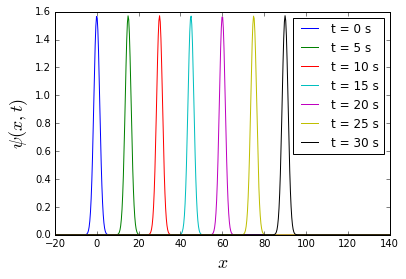
\includegraphics[scale=.6]{wave_packet_w_eq_kc.png}
\end{minipage}
\begin{minipage}{.5\textwidth}
\center
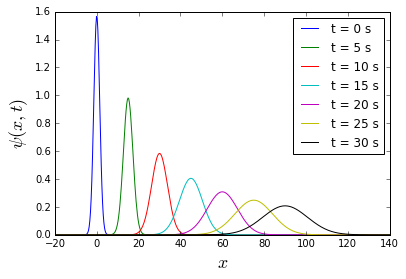
\includegraphics[scale=.6]{wave_packet_w_eq_function_of_k.png}
\end{minipage}
\caption{$\omega(k)/k$ sabitken ve $k$'nın bir fonksiyonu iken Denk. \ref{eq:wave_packet_t_approx} ile hesaplanan $|\psi(x,t)|^2$'nin değişimi.}
\label{fig:wave_packet_t}
\end{figure}

\subsection{Dalga Fonksiyonunun Olasılık Yorumu}

Çift yarık deneyinde bir fotonun kendi kendisiyle girişimini de izah eden toplam dalga fonksiyonunun karesinin fotonun, arka plandaki ekranda, belirli bir konum ve zamanda bulunma olasılığıyla orantılı olduğunu belirtmiştik. Benzetim yaparak $\psi(r,t)$ dalga fonksiyonuyla tanımlanan bir kuantum nesne içinde $|\psi(r,t)|$'nin bu nesnenin belirli bir konumda ve zamanda bulunma olasılığıyla ilişkili olduğunu iddia edebiliriz. Dalga fonksiyonunun olasılık yorumunu ilk ortaya koyan Max Born'dur. Max Born'a göre tek (iki, üç) boyutlu bir uzayda bir kuantum nesnenin (örneğin elektronun) $x$ ile $x+dx$ konumları arasında bulunma olasılığı,
%%
\begin{equation}
P(x,t) dx \equiv |\psi(x,t)|^2 dx
\label{eq:probability_interp}
\end{equation}
ile tanımlanır. Bu yoruma göre $|\psi(x,t)|^2$ zamanla yayılması, dalga fonksiyonu tarafından tanımlanan, ilgili kuantum nesnenin (elektron v.b.) ilerleyen zamanla birlikte artan ihtimalle başlangıçta bulunduğu bölgenin dışında bulunacaktır (bkz. Şekil \ref{fig:wave_packet_t}).

Kuantum fiziğinde olasılık kavramı klasik fiziktekinden farklıdır. Örneğin bir madeni paranın fırlatılmasıyla yazı mı, tura mı geleceğini bilememizin nedeni klasik fizikte sistem hakkındaki bilgimizin yetersizliği olarak belirtilir (ortamdaki hava moleküllerinin tek tek bireysel olarak para yüzeyi ile etkileşmerini ölçmek (bilmek) zordur v.b. gibi). Fakat kuantum fiziğinde ihtimaliyet bilgi eksikliğinden değil, dalga fonksiyonu hakkında bilebileceklerimizin temel bir sınırlamasından kaynaklanır.

Olasılık yoğunluğu yorumu çift yarık deneyindeki elektron girişiminin izahı için kullanılırsa, $\psi_1$ ve $\psi_2$ sırasıyla birinci yarık açık ikinci yarık kapalıykenki ve tersi durumdaki dalga fonksiyoları olmak üzere, arkadaki ekranda elektronların bulunma ihtimaliyetleri,
%%
\begin{equation}
P(x,t)^2 = |\psi_1 + \psi_2|^2 = |\psi_1 |^2 + |\psi_2|^2 + 2\text{Re}(\psi_1 + \psi_2^*)
\label{eq:interference_probability}
\end{equation}
%%
ile orantılıdır. Çünkü en sondaki terim olmadan girişim deseni izah edilemez. Bu nedenle $\psi_1$ ve $\psi_2$ için kurulacak olan diferansiyel denklem çizgisel olmalıdır ve dalga fonksiyonlarının üst üste gelmesi kuralına uygun olmalıdır.

Girişim desenini izah eden bu sonuç her zaman gözlenemeyebilir. Eğer yarıklardan birini kapatarak elektronları sadece bir yarıktan geçmeye zorlarsak ve böylece bir elektronun hangi yarıktan geçtiğini bilirsek elde edeceğimiz olasılık dağılımı,
%%
\begin{equation}
P(x,t)^2 = |\psi_1 |^2 + |\psi_2|^2
\label{eq:classical_probability}
\end{equation}
%%
olur. Bu durumda girişim deseni gözlenemez. Demek ki; girişim desenini gözleyebilmek için, elektronların geçtikleri yarıkların bilinmemesi gerekmektedir. Böylece şöyle bir sonuca varılabilir, \emph{eğer elektronların hangi yarıktan geçtiği biliniyorsa dalga fonksiyonlarının kareleri toplanarak, aksine hangi yarıktan geçtikleri bilinmiyorsa dalga fonksiyonlarının toplamlarının karesi alınarak olasılık dağılımları bulunur.}


\subsection{Schrödinger Denklemi}

Buraya kadar serbest hareket eden bir elektronun x konumunda ve t anında bulunma olasılığını tanımlayan bir dalga fonksiyonu tanınmadık. Planck'ın $E=\hbar\omega$  ve de~Broglie'nin $p=\hbar k$  ($\lambda = h/p$ )  bağlantılarını kullanarak  dalga fonksiyonunun kuantum fiziği ile bağını kurabiliriz.  Bu tanımlamalar ile dalga paketini,
%%
\begin{equation}
\psi \left( x,t\right) =\dfrac {1}{\sqrt {2\pi \hbar }}\int ^{\infty }_{-\infty }dp\phi \left( p\right) e^{i\left( px-Et\right) /\hbar }
\label{eq:wave_packet_in_p}
\end{equation}
%%
şeklinde yeniden yazabiliriz.  Burada A(k)'nın  yerini $\frac{\phi(p)}{2\pi\hbar}$  almıştır.  Serbest bir parçacığın toplam enerjisi
%%
\begin{equation}
E=\dfrac {p^{2}}{2m}
\label{eq:free_particle_E}
\end{equation}
%%
ile tanımlanır.  Enerji ifadesi,  Momentum ve grup hızı arasında
%%
\begin{equation*}
v_{g}=\dfrac {\partial \omega }{\partial k}=\dfrac {\hbar }{\hbar }\dfrac {\partial \omega }{\partial k}=\dfrac {\partial\hbar \omega }{\partial \hbar k}=\dfrac {\partial E}{\partial p}=\dfrac {p}{m}
\end{equation*}
%%
bağıntısı ortaya çıkar.  Böylece $E=\hbar \omega$ seçimimizin doğru olduğunu iddia edebiliriz. 

Eğer ilgilendiğimiz parçacık serbest olmasaydı toplam enerji
%%
\begin{equation}
E=\dfrac {p^{2}}{2m} + V(x)
\label{eq:non_free_particle_E}
\end{equation}
%%
olurdu.  Eğer bu ifadeyi doğrudan Denk.\ref{eq:wave_packet_in_p}'de yerine koyarsak çok anlamlı bir sonuç elde edemeyiz.  Çünkü dalga paketine sadece,
%%
\begin{equation*}
\text{e}^{iV\left( x\right) /\hbar }
\end{equation*}
%%
katkısı gelir.  Bu durumda $V(x)$'in  tanımladığı potansiyelin parçacık üzerindeki etkisini göremeyiz.  Çünkü
%%
\begin{equation*}
\left| \psi \left( x,t\right) \right| ^{2}\sim e^{iV\left( x\right) /\hbar }e^{-iV\left( x\right) /\hbar }=1
\end{equation*}
%%
olur. Bu sonuca göre elektron $V(x)$  potansiyelinden  etkilenmeden serbestçe hareket eder ki,  bu doğru bir  sonuç değildir. Yapılması gereken $V(x)$'in etkisini de hesaba katacak bir denklem geliştirmektir.

Eğer Denk. \ref{eq:wave_packet_in_p} ile tanımlanan dalga paketinin zamana göre türevini alırsak,
%%
\begin{align}
i \hbar \frac { \partial \psi ( x , t ) } { \partial t } &= \frac { 1 } { \sqrt { 2 \pi \hbar } } \int _ { - \infty } ^ { \infty } d p \phi ( p ) E ( p ) e ^ { i ( p x - E ) / \hbar } \nonumber\\
&= \frac { 1 } { \sqrt { 2 \pi \hbar } } \int _ { - \infty } ^ { \infty } d p \phi ( p ) \frac { p ^ { 2 } } { 2 m } e ^ { i ( p x - E t ) / \hbar }
\end{align}
%%
elde ederiz. Konuma göre birinci ve ikinci dereceden türevlerini alırsak,
%%
\begin{align}
\frac { \hbar } { i } \frac { \partial } { \partial x } \psi ( x , t ) = \frac { 1 } { \sqrt { 2 \pi \hbar } } \int _ { - \infty } ^ { \infty } d p \phi ( p ) p e ^ { i ( p x - E i )/\hbar }\nonumber\\
\left( \frac { \hbar } { i } \frac { \partial } { \partial x } \right) ^ { 2 } \psi ( x , t ) = \frac { 1 } { \sqrt { 2 \pi \hbar } } \int _ { - \infty } ^ { \infty } d p \phi ( p ) p ^ { 2 } e ^ { i ( p x - E i )/ \hbar }
\end{align}
%%
elde ederiz. Zamana ve konuma göre türevlerden elde ettiğimiz bu sonuçları birleştirirsek,
%%
\begin{equation}
i\hbar \dfrac {\partial \psi \left( x,t\right) }{\partial t}=-\dfrac {\hbar ^{2}}{2m}\dfrac {\partial ^{2}\psi \left( x,t\right) }{\partial x^{2}}
\label{eq:schrodinger_eq_free_particle}
\end{equation}
serbest bir parçacığın \emph{Schrödinger denklemi} olarak adlandırılan diferansiyel denkleme ulaşırız.
Denklemi serbest parçacığın klasik enerjisi (Denk. \ref{eq:free_particle_E}) ile kıyaslarsak $E$ ve $p$'nin yerini  sırasıyla $i \hbar \frac { \partial } { \partial t }$ ve $- i \hbar \frac { \partial } { \partial x }$ ifadelerinin aldığını söyleyebiliriz. Bu benzetmeyi serbest olmayan bir parçacığın klasik enerji ifadesi (Denk. \ref{eq:non_free_particle_E}) ile de yaparsak,
%%
\begin{equation}
i\hbar \dfrac {\partial \psi \left( x,t\right) }{\partial t}=-\dfrac {\hbar ^{2}}{2m}\dfrac {\partial ^{2}\psi \left( x,t\right) }{\partial x^{2}}+V\left( x\right) \psi \left( x,t\right)
\label{eq:schrodinger_eq}
\end{equation}
%%
serbest ve serbest olmayan parçacıkları tanımlayabileceğimiz, daha genel bir Schrödinger denklemi yazmış oluruz.

\subsubsection{$\phi\left(p\right)$  ve $\psi\left( x,0\right)$ Arasındaki İlişki}

Serbest parçacık durumunu düşünecek olursak, Schrödinger denkleminin en genel çözümü $\phi(p)$'nin şekline (davranışına) bağlıdır. $\phi(p)$'nin şeklini ise $t=0$ anındaki dalga paketi $\psi(x,0)$,
%%
\begin{equation}
\psi \left( x,0\right) =\dfrac {1}{\sqrt {2\pi \hbar }}\int ^{\infty }_{-\infty }dp\phi \left( p\right) e^{i px /\hbar }
\label{eq:wave_packet_in_t0}
\end{equation}
%%
integrali ile belirler. Bu integral aslında bir Foruier dönüşümü integralidir ve aşağıdaki yöntemle ters Foruier dönüşümü yapılırsa,
%%
\begin{equation}
\int _ { - \infty } ^ { \infty } d x \psi ( x , 0 ) e ^ { - i p ^ { \prime } x / \hbar } = \frac { 1 } { \sqrt { 2 \pi \hbar } } \int _ { - \infty } ^ { \infty } d x \int _ { - \infty } ^ { \infty } d p \phi ( p ) e ^ { i \left( p - p ^ { \prime } \right) x / \hbar }
\label{eq:wave_packet_in_p_t0}
\end{equation}
%%
ve $\int _ { - \infty } ^ { \infty } d x e ^ { i \left( p - p ^ { \prime } \right) x/\hbar } = 2 \pi \hbar \delta \left( p - p ^ { \prime } \right)$ olduğundan faydalanılırsa eşitliğin sol tarafı $\sqrt { 2 \pi  \hbar } \phi \left( p ^ { \prime } \right)$ olur. Böylece,
%%
\begin{equation}
\phi ( p ) = \frac { 1 } { \sqrt { 2 \pi \hbar } } \int _ { - \infty } ^ { \infty } d x \psi ( x , 0 ) e ^ { - i p x/ h }
\end{equation}
%%
sonucuna ulaşılır. 

\subsection{Heisenberg'in Belirsizlik Bağıntıları}

Hatırlanırsa dalga paketinin konuma ve dalga sayısına göre dağılımlarının genişliklerinin çarpımından Denk. \ref{eq:del_x_k}'i elde etmiştik. Bu bağıntı Foruier türü integrallerin daha genel bir sonucu olan,
\begin{equation}
\Delta k\Delta x >\dfrac {1}{2}
\end{equation}
ifadesinin özel bir halidir. $p = \hbar k$ bağıntısı ve dalga paketininin momentum uzayında da bir karşılığı olduğu hatırlanırsa yukarıdaki ifade,
%%
\begin{equation}
\Delta x \Delta p \geq\dfrac {\hbar}{2}
\label{eq:heisenberg_uncertainty}
\end{equation}
%%
halini alır ve Heisenberg belirsizlik bağıntısı olarak adlandırılır. Dalga paketlerinin incelenmesi sonucu elde ettiğimiz bu eşitliğin sayesinde anlıyoruz ki; dalga fonksiyonu hem konumu hem de momentumu çok keskin bir doğrulukla veremez. Klasik mekanikteki anlayışımıza ters bir durumdur. Bu eşitlik klasik kavramlar olan konum ve momentumun doğru ölçülmesinde kuantum sistemlerin doğasından kaynaklanan bir sınırlama olduğunu göstermektedir. Klasik fizikteki gibi konum ve momentumun birbirinden bağımsız olacağını söylemek artık mümkün değildir. Bu nedenle bu tür fiziksel nicelikler tümleyen değişkenler olarak adlandırılır.  Kauntum fiziğinin doğasındaki bu sınırlamalar ile ilgili aşağıda örnek verilmiştir.  

\subsubsection{Bir Foton Demetinin Kırınımı}

\href{https://opentextbc.ca/physicstestbook2/chapter/single-slit-diffraction/}{Tek yarık kırınımı}

\begin{figure}[hbtp]
	\centering
	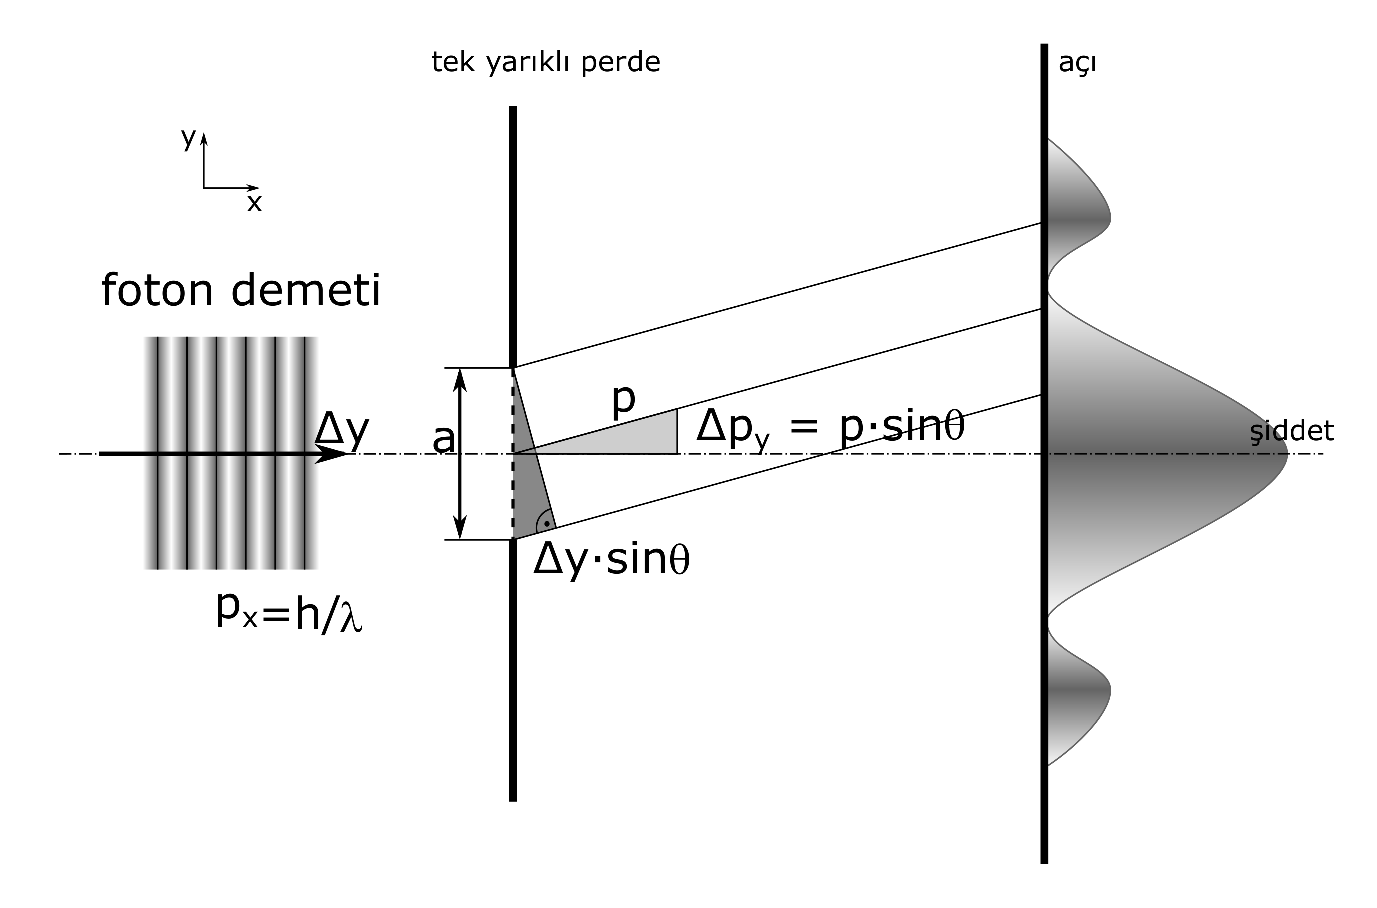
\includegraphics[width=0.7\linewidth]{figurler/tek_yarik_deneyi.eps}
	\caption{Tek yarıktan geçen ve kırınıma uğrayan foton demeti}
	\label{fig:tekyarikdeneyi}
\end{figure}

Şekil \ref{fig:tekyarikdeneyi}'teki gibi bir tek yarıklı filtreye foton demeti gönderdiğimizi düşünelim. Foton demetinin dalga davranışı gösterdiğini düşünecek olursak, şekildeki gibi bir kırınım deseni oluşturarak dağılacaktır. Bu dağılmanın miktarını,
%%
\begin{equation*}
\theta \eqsim \frac{\lambda}{a}
\end{equation*}
%%
ifadesi belirler. Dalga parçacık ikileminin bir sonucu olarak foton demetini aynı yarıktan geçen parçacıklar olarak da düşünmek mümkündür. Eğer foton parçacıklarının momentumlarını ve konumlarını kesin bir doğrulukla bilebilseydik, foton demetinin dağılması gerçekleşmezdi. Fakat fotonu parçacık olarak da düşünsek, dalga olarak da düşünsek bu dağılım gerçekleşmektedir. 

Burada bir paradoks varmış gibi görünmekle beraber, bizi bu sözde paradokstan kurtaran Heisenberg'in belirsizlik bağıntısıdır. Fotonlar $x$ doğrultusunda $p_x~=~h/\lambda$ momentumuna sahip olacak şekilde bir kaynaktan çıkıyor olsunlar. $y$ doğrultusundaki konumlarını,
%%
\begin{equation*}
\Delta y \leq a
\end{equation*}
%%
aralığıyla sınırlı bir belirsizliği içerecek kadar bilebiliriz. Bu durumda yarıktan geçtikten sonraki $y$ doğrultusundaki momentumları Heisenberg'in bağıntsına göre,
%%
\begin{equation*}
\Delta p_y \geq \frac{h}{\Delta y}>\frac{h}{a}
\end{equation*}
%%
civarında bir belirsikliğe sahip olur. Yarıktan geçmeden önce fotonlar sadece $p_x$ momentumlu iken sonrasında $\Delta p_y$ belirsizliği civarındaki ve $y$ doğrultusundaki momentumlara sahip olacaklardır.
$\Delta p_y$'yi başlangıçtaki $p_x$ momentumundan sapma miktarı gibi düşünürsek ve $p$'yi yarıktan sonraki toplam momentum olarak tanımlarsak, her iki doğrultadki momentumların bir birine oranı demetin dağılma miktarı hakkında bilgi verecektir. Buna göre,
%%
%%
\begin{align}
\frac{\Delta p_y}{p_x} &= \frac{p \sin\theta}{p \cos\theta}\eqsim\theta \text{ (çok küçük açılar için)}\\
\frac{\Delta p_y}{p_x} &\approx \frac { h / a } { h / \lambda } \approx \frac { \lambda } { a }
\end{align}
olur. Böylece foton demetini elektromanyetik dalga olarak incelediğimiz durumdaki dağılımın parçacık durumu içinde geçerli olduğunu göstermiş oluruz.


\subsubsection{Bohr Yörüngelerinin Yerelleşememesi}
%%
Kuantum fiziğine göre; bir elektronun bağlı bulunduğu atom etrafındaki klasik bir kapalı yörüngede hareket etmesi kavramı anlamını yitirmiştir. Çünkü bir elektronun bir kapalı yörüngeyi izlediğini söyleyebilmek için o yörünge üzerinde elektron yörüngeyi tamamlayana kadar elektronu izlemek gerekir. Böyle bir izlemenin yapabilmesi için elektronun yörünge üzerindeki herhangi bir andaki konumunun büyük bir kesinlikle bilinmesi gerekir.

Geçici olarak, Bohr'un varsayımlarına göre bir dairesel yörüngeyi izlediğini iddia ettiğimiz bir elektronu düşünelim. Böyle bir elektronun yörünge üzerinde hangi konumda bulunduğu ölçebilmek için üzerine bir foton göndermeliyiz. Böyle bir fotonun dalga boyunun atomun klasik yörüngelerini çözme gücüne sahip olması gerekir, diğer bir deyişle fotonun dalga boyu iki klasik yörünge arası mesafeden küçük olması gerekir. Bohr'un varsayımlarından yola çıkarak elde ettiğimiz yörünge yarıçapı ifadesini iki yörünge arasındaki uzaklığı bulmak için,
%%
\begin{equation*}
r _ { n + 1 } - r _ { n } = \frac { \hbar } { m _ { e } c \alpha } \left[ ( n + 1 ) ^ { 2 } - n ^ { 2 } \right] = \frac { \hbar } { m _ { e } c \alpha } (2n+1) \approx \frac { \hbar } { m _ { e } c \alpha } n
\end{equation*}
%%
kullanabiliriz. Aradığımız çözünürlüğe ulaşabilmek için fotonun dalga boyu bu uzaklıktan küçük olmalıdır,
%%
\begin{equation*}
\lambda << r _ { n + 1 } - r _ { n }.
\end{equation*}
%%
Böyle bir fotonun momentumu ise,
%%
\begin{equation*}
p_{ \gamma } \approx \frac { h } { \lambda } >> \frac { m _ { e } c \alpha } { 2\pi n }
\end{equation*}
%%
olur ki, bu momentumun tamamının konumunu bilmek istediğimiz elektrona aktarıldığını düşünelim. Elektronun enerjisindeki değişim yaklaşık olarak veya elektrona aktarılan enerji,
%%
\begin{align*}
E = \frac{p^2}{2m_e} \Rightarrow \Delta E &\approx \frac { p \Delta p } { m _ { e } } \approx \frac { p p _ { \gamma } } { m _ { e } } = \frac{(m_e c) (m_e c \alpha/2\pi n)}{m_e}\\
&\approx \frac { m_e c^2 \alpha} { 2\pi n } >> \frac { m _ { e } ( c \alpha ) ^ { 2 } } { n ^ { 2 } }
\end{align*}
%%
hesaplamalarıyla bulunur ki, bu enerji yukarıdaki ifadelerden anlaşılacağı üzere elektronun bağlanma enerjisinden çok daha büyüktür. Böyle bir enerji ile konumunu bilmek istediğimiz elektronu yörüngesinden çıkarmış oluruz. Ortaya çıkan sonuca göre konumunu yüksek kesinlikle bilmek istediğimiz sistemin, momenumu hakkındaki bilgi edinme kabiliyetimizi büyük ölçüde zayıflatmış oluruz. Böylece Heisenberg'in belirsizlik bağıntısının bir kere daha doğrulandığını söyleyebiliriz.

\subsection{Dalga Fonksiyonun ve Olasılığın Normalizasyonu}

\begin{equation}
\int ^{\infty }_{-\infty }dxP\left( x,t\right) =\int ^{\infty }_{-\infty }dx\left| \psi \left( x,t\right) \right| ^{2}=1
\label{eq:probability_norm}
\end{equation}
%%

Olasılık yorumuna göre toplam olasılığı veren yukarıdaki integralin  sonucu sonlu bir değer vermelidir.  Elde edilen integral sonucu birim değere sahip değilse, gelenek olduğu üzere toplam olasılık $1$'e normalize edilir.  Normalizasyon sonucu  elde edilen katsayı ile dalga fonksiyonu çarpılır, böylece elde edilen yeni dalga fonksiyonu da Schrödinger denkleminin bir çözümüdür. Çünkü dalga denklemi çizgiseldir. Yeni dalga fonksiyonuna normalize edilmiş dalga fonksiyonu denir.

Böylece bir kuantum durumu izah edecek başlangıç durumu dalga fonksiyonunun \emph{``karesi integrallenebilir"} bir fonksiyon olması gerekir. 
%%
\begin{equation}
\int ^{\infty }_{-\infty }dx\left| \psi \left( x,0\right) \right| ^{2} < \infty
\label{eq:square_integrable}
\end{equation}
%%
Karesi integrallenebilir olma şartının matematiksel ifadesi yukarıdaki gibidir. İleride konum ($x$) ve konuma göreve türev ($\partial/\partial x$) içeren bir çok integralle karşılaşacağız. Örneğin,
%%
\begin{equation*}
\int ^{\infty }_{-\infty }dx \psi^* \left( x,t\right) x^n \psi \left( x,t\right) 
\end{equation*}
%%
ve
%%
\begin{equation*}
\int ^{\infty }_{-\infty }dx \psi^* \left( x,t\right) \left(\frac{\partial}{\partial x}\right)^n \psi \left( x,t\right) 
\end{equation*}
%%
gibi, bu integrallerin karesi integrallenebilir olması için $\psi(x,0)$ başlangıç durumu dalga fonksiyonunun $x\rightarrow\pm\infty$ ile hızlıca sıfıra gitmesi gerekir. Ayrıca $\psi(x,t)$ $x$'in sürekli bir fonksiyonu olmalıdır.

\subsubsection{Olasılık Akısının Tanımı ve Önemi}

%% Aşağıdaki denklemler
%% https://webdemo.myscript.com/views/main/math.html
%% linkindeki el yazısı tanıyan program kullanırak yazıldı.

Dalga fonksiyonunu $t=0$ anında normalize etmekle, herhangi bir t anında da dalga fonksiyonunu normalize etmiş olur muyuz? Soruyu olumlu cevaplayabilmek için 
\begin{equation}
\dfrac {\partial }{\partial t} \int ^{\infty }_{-\infty }dxP\left( x,t\right) = \dfrac {\partial }{\partial t} \int ^{\infty }_{-\infty }dx\left| \psi \left( x,t\right) \right| ^{2}= \dfrac {\partial }{\partial t}N(t) \stackrel{\scalebox{2}{?}}{=} 0 
\label{eq:probability_norm_derivative}
\end{equation}
%%
Denk. \ref{eq:probability_norm}'in zamana göre kısmi türevi olan yukarıdaki ifadenin belli şartlarda sıfıra eşit olabileceğini göstermek gerekir. Eğer eşitlik sağlanırsa $N(t) = \text{sabit}$ olur. Böylece dalga fonksiyonu herhangi bir $t$ anında normalize edilebilir. Yukarıdaki eşitliği sorgulamak için öncelikle $P(x,t)$ olasılık yoğunluğunun $t$'ye göre kısmi türevi alınırsa,
%%
\begin{equation}
\dfrac {\partial }{\partial t}P\left( x,t\right) = \dfrac {\partial \psi ^{\ast }}{\partial t}\psi +\psi ^{\ast }\dfrac {\partial \psi }{\partial t}
\label{eq:probability_derivative_t}
\end{equation}
%%
elde edilir. Elde edilen bu eşitliğin sağ tarafında Schrödinger denklemi ve onun karmaşık eşleniği olan,
\begin{equation}
-i\hbar \dfrac {\partial \psi ^{\ast }\left( x,t\right) }{\partial t}=-\dfrac {\hbar ^{2}}{2m}\dfrac {\partial ^{2}\psi ^{\ast }\left( x,t\right) }{\partial x^{2}}+V\left( x\right) \psi ^{\ast }\left( x,t\right)
\label{eq:schrodinger_conjugate}
\end{equation}
hali kullanılırsa ve $V(x)$'in reel bir fonksiyon olduğu kabul edilirse,
%%
\begin{align}
\dfrac {\partial }{\partial t}P\left( x,t\right) &=\dfrac {1}{i\hbar }\left( \dfrac {\hbar ^{2}}{2m}\right) \left( \dfrac {\partial ^{2}\psi ^{\ast }}{\partial x^{2}}\psi -\psi ^{\ast }\dfrac {\partial ^{2}\psi }{\partial x^{2}}\right) \\
%%
&=-\dfrac {\partial }{\partial x}\left[ \dfrac {\hbar }{2im}\left( \psi ^{\ast }\dfrac {\partial \psi }{\partial x}-\dfrac {\partial \psi ^{\ast }}{\partial x}\psi \right) \right]
\end{align}
%%
sonucuna ulaşılır. Burada eşitliğin sağında türevin içinde kalan kısımı \emph{olasılık akısı} olarak tanımlanır,
%%
\begin{equation}
j(x,t)\equiv \dfrac {\hbar }{2im}\left( \psi ^{\ast }\dfrac {\partial \psi }{\partial x}-\dfrac {\partial \psi ^{\ast }}{\partial x}\psi \right).
\label{eq:probability_current}
\end{equation}
%%
Bu tanımla olasılık yoğunluğunun zamana göre değişimini veren denklem,
\begin{equation}
\dfrac {\partial }{\partial t}P\left( x,t\right) +\dfrac {\partial }{\partial x}j\left( x,t\right) =0
\label{eq:continuity_equation}
\end{equation}
halini alır. Süreklilik denklemi olarak da adlandırılan denklemin $x$'e göre integrali alınırsa,
%%
\begin{equation}
\dfrac {\partial }{\partial t}\int ^{\infty }_{-\infty }dxP\left( x,t\right) =-\int ^{\infty }_{-\infty }dx\dfrac {\partial }{\partial x}j\left( x,t\right) = -j(x,t)\bigg|^{\infty}_{-\infty}
\end{equation}
sonucu elde edilir. Bu son eşitliğin en sağ tarafı sıfıra eşit olursa, aradığımız sonuca ulaşımış oluruz. Aranan sıfırın elde edilmesi için \emph{olasılık aksının} denklemini incelemek gerekir: denklemde dalga fonksiyonunun (ve eşleniğinin) kendisi ve birinci türevi vardır. Eğer $x\rightarrow\pm\infty$ durumunda dalga fonksiyonu ve eşleniği sıfıra giderse ve birinci türevleri de sabit değerli kalırsa aranılan sonuca ulaşılabilir. Böylece Denk. \ref{eq:probability_norm_derivative}'nın bu şartlar altında sağlanacağı ve bu şartlara uyan dalga fonksiyonlarının herhangi bir $t$ anında normalize edilebileceği gösterilmiş olur. 

\vspace{18pt}
{\bf ``MIT Açık Dersler"den güzel bir video dersi kaynağı:}

\href{https://ocw.mit.edu/courses/physics/8-04-quantum-physics-i-spring-2016/video-lectures/part-1/}{Lecture 6: Probability density and current. Hermitian conjugation.}


\subsection{Konum ve Momentum Beklenen Değerleri}

Heisenberg'in belirsizlik bağıntıları kavramını incelerken anladığımız üzere bir parçacığın konum veya momentumunu kesin olarak bilmemiz mümkün değildir. Bunun yerine belirli olasılıklarla hangi değerler civarında konuma ve momentuma sahip olabileceği hakkında konuşabiliriz. Böyle bir olasılığı hesaplamak için, bir sınavda alınan notların standart sapmasını belirlemek için kullandığımız yönteme benzer bir yöntem geliştirmeliyiz \cite{book:Towsend}.

Genellikle sınavlarda bilinmek istenen ilk şey: Sınavın not ortalaması nedir? Bütün sınavın not toplamını sınava giren toplam kişi sayısına bölersek bu ortalamayı rahatça buluruz. Eş değer olarak aşağıdaki gibi bir olasılık dağılımı oluşturabiliriz,
%%
\begin{equation}
P\left( n\right) =\dfrac {N(n) }{N}
\label{eq:probability_distrubition_P}
\end{equation}
%%
Burada $N(n)$, $n$ notunu alanların sayısı ve $N$ sınıf mevcududur. Eğer not aralığı $0\leq n \leq 100$ ile tanımlanmışsa $P(n)$,
%%
\begin{equation}
\sum ^{100}_{n=0}P\left( n\right) =\sum ^{100}_{n=0}\dfrac {N(n) }{N}=\dfrac {1}{N}\sum ^{100}_{n=0}N(n) =1
\label{eq:normalization_P}
\end{equation}
%%
normalizasyon şartını sağlamalıdır. Böylece sınavın ortalaması,
%%
\begin{equation}
\langle n \rangle =\dfrac {1}{N}\sum ^{100}_{n=0}nN\left( n\right) =\sum ^{100}_{n=0}nP\left( n\right) 
\label{eq:average_grade}
\end{equation}
%%
olur. Ortalamanın yanında ortalama etrafındaki dağılım bilgisini veren \emph{standart sapma}yı da bilmek sınavın not dağılımı hakkında daha çok bilgi edinilmesini sağlar. Tek bir sınav notu için standart sapma,
%%
\begin{equation}
\sigma ^{2}_{n}\equiv(n-\langle n\rangle) ^{2}
\label{eq:standard_deviation_atom}
\end{equation}
%%
ile tanımlanır. Bütün sınavın standart sapması ise bireysel standart sapmaların ortalamsıdır ve,
\begin{equation}
\sigma ^{2}\equiv \langle \left( n-\langle n\rangle \right) ^{2}\rangle =\sum ^{100}_{n=1}\sigma _{n}^2P\left( n\right) 
\label{eq:standard_deviation_exam}
\end{equation}
ile tanımlanır. Aşağıdaki gibi bir kaç düzenleme ile,
\begin{align*}
\sigma ^{2}=\sum ^{100}_{n=0}\sigma ^{2}_{n}P\left( n\right) &=\sum ^{100}_{n=0}\left(n -\langle n\rangle \right) ^{2}P\left( n\right) \\
&=\sum ^{100}_{n=0}\left( n^{2}P\left( n\right) -2n\langle n\rangle P\left( n\right) +\langle n\rangle ^{2}P\left( n\right) \right)\\
&=\sum ^{100}_{n=0}n^{2}P\left( n\right) -2 \langle n \rangle\sum ^{100}_{n=0}nP\left( n\right) +\langle n\rangle ^{2}\sum ^{100}_{n=0}P\left( n\right) \\
&=<n^{2}>-2 \langle n \rangle\langle n\rangle +\langle n\rangle ^{2}\\
\end{align*}
%%
kısaca,
%%
\begin{equation}
\sigma^2 = \langle n^{2}\rangle - \langle n \rangle^{2}
\end{equation}
%%
olarak yazılabilir. Böylece sınavdaki notların,
\begin{equation*}
\langle n \rangle - \sigma \leq n \leq \langle n \rangle + \sigma
\end{equation*}
ifadesine göre $\langle n \rangle$ ortalaması etrafında dağılım gösterdiklerini söyleyebiliriz. Notların az bir kısmı bu aralık dışında kalabilir.

Benzeri bir uygulamayı ilgilendiğimiz parçacığın konumu ve momentumu için de yapabiliriz. Örneğin konum ($x$) veya konumun bir fonksiyonu ($f(x)$) için ortalama değer,
%%
\begin{equation}
\langle f(x) \rangle =\int ^{\infty }_{-\infty }dx f(x) P\left( x,t\right) =\int ^{\infty }_{-\infty }dx \psi^{\ast }\left(x,t\right) f(x) \psi \left( x,t\right)
\label{eq:expactation_value}
\end{equation}
olarak yazılabilir. Bu ortalama değer genellikle \emph{beklenen değer} olarak adlandırılır. Beklenen değer ifadesinden aynı fiziksel olayın gerçekleştirilen bir dizi deneyinde ölçüm sonuçlarının her zamana $\langle f(x) \rangle$ sonucunu vereceği anlaşılmamalıdır. Ölçümlerin sonuçlarının beklenen değer etrafında $\Delta f(x) = \sqrt{\langle f(x)^2 \rangle - \langle f(x) \rangle^2}$ standart sapmasına göre dağılmaları beklenir. Kuantum fiziğindeki standart sapmanın integral formu aşağıdaki gibidir.
%%
\begin{equation}
\Delta f(x)^2 = \int ^{\infty }_{-\infty }dx \psi^{\ast }\left(x,t\right) f(x)^2 \psi \left( x,t\right) -\left( \int ^{\infty }_{-\infty }dx \psi^{\ast }\left(x,t\right) f(x) \psi \left( x,t\right)\right)^2
\end{equation}
%%
Bir parçacığın konumu için beklenen değeri ve standart sapmayı bulmak kolaydır, $f(x)$ yerine $x$ koymak yeterlidir. 

Parçacığın momentumunun beklenen değeri için nasıl bir yol izleyeceğimiz çok açık değildir. P. Ehrenfest \emph{uygunluk prensibi}nden faydalanarak,
%%
\begin{equation*}
p = m v = m\frac{dx}{dt}
\end{equation*}
%%
klasik ifadesinin,
%%
\begin{equation*}
\langle p \rangle = m\frac{d \langle x \rangle}{dt}
\end{equation*}
%%
olarak kullanılabileceğini göstermiştir. Buradan yola çıkarak,
%%
\begin{align}
\langle p \rangle &= m \frac{d}{dt} \int ^{\infty }_{-\infty }dx \psi^{\ast }\left(x,t\right) x \psi \left( x,t\right)\\
&=m\int ^{\infty }_{-\infty }dx\left( \dfrac {\partial \psi ^{\ast }\left( x,t\right) }{\partial t}x\psi \left( x,t\right) +\psi ^{\ast }\left( x,t\right) x \dfrac {\partial \psi \left( x,t\right) }{\partial t}\right) \nonumber 
\end{align}
%%
yazılabilir. Bu hesapta $dx/dt$ türev ifadesinin yer almadığına dikkat edilmelidir. Zamana bağlı olan ifade $\psi(x,t)$ ve onun eşleniğidir. Dalga fonksiyonunun zamanla değişimi $\langle x \rangle$'deki zamana bağlı değişimi belirler. Olasılık akısını hesaplarken yaptığımız gibi yukarıdaki denklemde Schrödinger denklemini ve eşleniğini kullanalarak,
%%
\begin{equation}
\langle p\rangle =\dfrac {\hbar }{2i}\int ^{\infty }_{-\infty }dx\left( \dfrac {\partial ^{2}\psi ^{\ast }}{\partial x^{2}}x\psi -\psi ^{\ast }x\dfrac {\partial ^{2}\psi }{\partial x^{2}}\right)
\label{eq:expectation_val_p_1}
\end{equation}
%%
sonucuna ulaşırız. Bu ifadeyi üzerinde biraz daha matematiksel çalışma yapmalıyız.
%%
\begin{align*}
\dfrac {\partial }{\partial x}\left( \dfrac {\partial \psi ^{\ast }}{\partial x}x\psi \right) =\dfrac {\partial ^{2}\psi^{\ast }}{\partial x^{2}}x\psi +\dfrac {\partial \psi ^{\ast }}{\partial x}\psi +\dfrac {\partial \psi ^{\ast }}{\partial x}x\dfrac {\partial \psi }{\partial x} \\
\dfrac {\partial }{\partial x}\left( \psi ^{\ast }x\dfrac {\partial \psi }{\partial x}\right) =\dfrac {\partial \psi ^{\ast }}{\partial x}x\dfrac {\partial \psi }{\partial x}+\psi ^{\ast }\dfrac {\partial \psi }{\partial x} + \psi ^{\ast } x \dfrac {\partial ^{2}\psi }{\partial x^{2}}
\end{align*}
%%
Yukarıdaki iki eşitlikten alttaki üsttekinden çıkarılırsa,
%%
\begin{equation*}
\left( \dfrac {\partial ^{2}\psi ^{\ast }}{\partial x^{2}}x\psi -\psi ^{\ast }x\dfrac {\partial ^{2}\psi }{\partial x^{2}}\right) = \dfrac {\partial }{\partial x}\left( \dfrac {\partial \psi ^{\ast }}{\partial x}x\psi -\psi ^{\ast }x\dfrac {\partial \psi }{\partial x}\right) +\psi ^{\ast }\dfrac {\partial \psi }{\partial x}-\dfrac {\partial \psi ^{\ast }}{\partial x}\psi 
\end{equation*}
%%
elde edilir. Eşitliğin sol tarafındaki son iki terim için de,
\begin{align*}
\dfrac {\partial \psi ^{\ast }\psi }{\partial x}=\dfrac {\partial \psi ^{\ast }}{\partial x}\psi +\psi ^{\ast }\dfrac {\partial \psi }{\partial x}\\
\dfrac {\partial \psi ^{\ast }}{\partial x}\psi =\dfrac {\partial \psi ^{\ast }\psi }{\partial x}-\psi ^{\ast }\dfrac {\partial \psi }{\partial x}
\end{align*}
bu matematiksel işlemin sonucu kullanılırsa $\langle p \rangle$ için,
%%
\begin{equation*}
\langle p\rangle =\dfrac {\hbar }{2i}\int ^{\infty }_{-\infty }dx\left( \dfrac {\partial ^{2}\psi ^{\ast }}{\partial x^{2}}x\psi -\psi ^{\ast }x\dfrac {\partial ^{2}\psi }{\partial x^{2}}\right) =  \dfrac {\hbar }{2i}\int ^{\infty }_{-\infty }dx \left[\dfrac {\partial }{\partial x}\left( \dfrac {\partial \psi ^{\ast }}{\partial x}x\psi -\psi ^{\ast }x\dfrac {\partial \psi }{\partial x} + \psi^\ast \psi\right) +2\psi ^{\ast }\dfrac {\partial \psi }{\partial x}\right]
\end{equation*}
%%
sonucuna ulaşılır. Bu ifadeyi biraz daha açarsak,
%%
\begin{equation*}
\langle p\rangle = \dfrac {\hbar }{2i}\left( \dfrac {\partial \psi ^{\ast }}{\partial x}x\psi -\psi ^{\ast }x\dfrac {\partial \psi }{\partial x} + \psi^\ast \psi \right){\bigg |}_{-\infty}^{\infty} + \int ^{\infty }_{-\infty }dx \psi ^{\ast }\left(\dfrac {\hbar }{i}\dfrac {\partial}{\partial x}\right) \psi
\end{equation*}
%%
momentumun beklenen değerini bulmaya daha da yakınlaşmış oluruz. Bu son ifadedeki ilk terimdeki dalga fonksiyonları ve eşlenikleri $\pm\infty$ durumları için sıfıra gideceklerinden ilk terim kaybolur ve momentumun beklenen değeri,
%%
\begin{equation}
\langle p\rangle =  \int ^{\infty }_{-\infty }dx \psi(x,t) ^{\ast }\left(\dfrac {\hbar }{i}\dfrac {\partial}{\partial x}\right) \psi(x,t)
\label{eq:expactation_value_and_op_momentum}
\end{equation}
%%
olarak bulunur. Burada klasik momentumun kuantum fiziğinde bir diferansiyel operatörle (işlemci) ile temsil edildiğini kabul ederiz ve bu operatörün,
%%
\begin{equation}
\hat p \equiv \dfrac {\hbar }{i}\dfrac {\partial}{\partial x}
\end{equation}
%%
ile tanımlarız. Bu tanımı kabullendiğimiz takdirde serbest bir parçacığın enerjisi için
%%
\begin{equation}
\hat E \equiv \dfrac{\hat p^2}{2 m} = \dfrac {1 }{2 m}\left(\dfrac {\hbar }{i}\dfrac {\partial}{\partial x}\right)^2 = -\dfrac {\hbar^2 }{2 m}\dfrac {\partial^2}{\partial^2 x}
\end{equation}
%%
yazılabilir. Böylece bir serbest parçacığın enerjisinin beklenen değeri,
%%
\begin{equation}
\langle \hat E\rangle =  \int ^{\infty }_{-\infty }dx \psi(x,t) ^{\ast }\left(-\dfrac {\hbar^2 }{2 m}\dfrac {\partial^2}{\partial^2 x}\right) \psi(x,t)
\label{eq:expactation_value_and_op_energy}
\end{equation}
%%
intergrali ile hesaplanabilir. Dikkat edilirse yeni tanımlandığımız bu operatörleri klasik ifadeden ayırmak için üzerine şapka sembolü ekliyoruz.

Momentum operatörünün $i$ sanal sayısını içeriyor olması beklenen değerin de bazen sanal sayı içerebileceğini düşünüdürebilir. Beklenen değerin sanal olup olmayacağını,
%%
\begin{equation}
\langle \hat p \rangle - \langle \hat p \rangle^\ast = 0
\end{equation}
%%
ifadesi ile test edebiliriz. Eğer eşitlik sağlanırsa $\langle \hat p \rangle$ reeldir. Çünkü, reel bir sayının eşleniği kendisine eşittir. Şimdi bu eşitliği test edelim.
%%
\begin{align*}
\langle \hat p \rangle - \langle \hat p \rangle^\ast &= \int ^{\infty }_{-\infty }dx \psi ^{\ast }\left(\dfrac {\hbar }{i}\dfrac {\partial}{\partial x}\right) \psi - \left(  \int ^{\infty }_{-\infty }dx \psi ^{\ast }\left(\dfrac {\hbar }{i}\dfrac {\partial}{\partial x}\right) \psi  \right)^\ast \\
&= \int ^{\infty }_{-\infty }dx \psi ^{\ast }\left(\dfrac {\hbar }{i}\dfrac {\partial}{\partial x}\right) \psi -   \int ^{\infty }_{-\infty }dx \psi \left(-\dfrac {\hbar }{i}\dfrac {\partial}{\partial x}\right) \psi^\ast \\
&= \dfrac {\hbar }{i} \int ^{\infty }_{-\infty }dx \left[\psi ^{\ast } \dfrac {\partial}{\partial x} \psi +  \psi \dfrac {\partial}{\partial x}\psi^\ast\right] = \dfrac {\hbar }{i} \int ^{\infty }_{-\infty }dx \dfrac {\partial}{\partial x}\left( \psi ^{\ast } \psi\right)\\
&=\psi^\ast \psi {\bigg |}^{\infty}_{-\infty} = 0
\end{align*}
%%
Bu teste göre eşitlik sağlanır, çünkü son elde edilen terimdeki dalga fonksiyonu ve eşleniği sonsuzda sıfıra gidecektir. Böylece momentumun beklenen değerinin daima reel olacağını söyleyebiliriz. Bu tür reel değerli beklenen değer üreten operatörlere \emph{hermityen operatörler} denir.

Elde ettiğimiz bu hermityen momentum operatörünü kullanarak Schrödinger denklemini,
%%
\begin{equation}
\hat H\psi(x,t) = i\hbar \dfrac{\partial}{\partial t}\psi(x,t)
\label{eq:schrodinger_operator_form}
\end{equation}
%%
operatör formunda yazabiliriz, burada $\hat H$ \emph{Hamiltonyen işlemcisi} olarak adlandırılır ve,
%%
\begin{equation}
\hat H \equiv \frac{\hat p^2}{2 m} + \hat V(x)
\label{eq:schrodinger_operator_form}
\end{equation}
%%
olarak tanımlanır.

\subsubsection{Momentum Uzayında Beklenen Değer}

Daha önce dalga paketini yerelleştirmek için kullandığımız $\phi(p)$ fonksiyonunun Foruier dönüşümü ile $\psi(x,0)$'dan aşağıdaki ifade ile elde edilebileceğini tartışmıştık.
%%
\begin{equation}
\phi \left( p\right) =\dfrac {1}{\sqrt {2\pi \hbar }}\int ^{\infty }_{-\infty }dx\psi \left( x,0\right) e^{-ipx/\hbar }
\end{equation}
%%
$\phi(p)$'yi yerelleşmeyi sağlaması dışında bir başka şekilde anlamlandırabilir miyiz? Önceklikle, \emph{Parseval teoremine} göre $\psi(x)$ normalize ise $\phi(p)$'de normalizedir. Aşağıdaki matematiksel işlem süreci her iki fonksiyondan birisi normalizeyse diğerininde normalize olacağını ispatlamaktadır.
%%
\begin{align}
\int ^{\infty }_{-\infty }dp\phi ^{\ast }\left( p\right) \phi \left( p\right) &=\int ^{\infty }_{-\infty }dp\phi ^{\ast }\left( p\right) \dfrac {1}{\sqrt {2\pi \hbar }}\int ^{\infty }_{-\infty }dx\psi \left( x\right) e^{-ipx/\hbar }\nonumber \\
&=\dfrac {1}{\sqrt {2\pi \hbar }}\int ^{\infty }_{-\infty }dx\psi \left( x\right) \int ^{\infty }_{-\infty }dp\phi^\ast \left( p\right) e^{-ipx/\hbar }\nonumber \\
&=\int ^{\infty }_{-\infty }dx\psi \left( x\right) \psi ^{\ast }\left( x\right) = 1
\label{eq:parseval_theorem}
\end{align}
%%
Şimdi benzer şekilde, Fourier dönüşümlerinden faydalanarak, $\langle \hat p \rangle$ beklenen değerini incelersek,
%%
\begin{align}
\langle \hat p\rangle &=\int ^{\infty }_{-\infty }dx\psi^\ast \left( x\right) \dfrac {\hbar }{i}\dfrac {\partial}{\partial x}\psi \left( x\right) =\int ^{\infty }_{-\infty }dx\psi^\ast \left( x\right) \dfrac {\hbar }{i}\dfrac {d}{dx}\dfrac {1}{\sqrt {2\pi \hbar }}\int ^{\infty }_{-\infty }dp\phi \left( p\right) e^{ipx/\hbar }\nonumber \\
&=\int ^{\infty }_{-\infty }dp\phi \left( p\right) \,p\, \dfrac {1}{\sqrt {2\pi x}}\int ^{\infty }_{-\infty }dx\psi ^{\ast }\left( x\right) e^{ipx/\hbar }\nonumber \\
&= \int ^{\infty }_{-\infty }dp\phi ^{\ast }(p)\,p\,\phi(p)
\label{eq:wave_in_momentum_space} 
\end{align}
%%
Denklem \ref{eq:parseval_theorem} ve \ref{eq:wave_in_momentum_space}'ya dayanarak $\phi(p)$'yi dalga fonksiyonunun momentum uzayındaki temsili olarak veya kısaca momentum uzayıdaki dalga fonksiyonu olarak tanımlayabiliriz. Böylece $|\phi(p)|^2$'yi de bir parçacığın p momentumuna sahip olma olasılık yoğunluğu olarak adlandırabiliriz. Konum uzayında konum operatörü basitçe $\hat x = x$ ve momentum operatörü $\hat p = \dfrac{\hbar}{i}\dfrac{\partial}{\partial x}$ ile tanımlanırken, momentum uzayında konum $\hat x = i \hbar\dfrac{\partial}{\partial p}$ ile momentum ise basitçe $\hat p = p$ ile tanımlanır. Böylece momentum uzayında konumun beklenen değeri,
%%
\begin{equation}
\langle \hat x \rangle =  \int ^{\infty }_{-\infty }dp\phi ^{\ast }(p)\left(i\hbar\dfrac{\partial}{\partial p}\right)\phi(p)
\end{equation}
%%
ifadesi ile hesaplanabilir.

\newpage
% In the preamble, add "\renewcommand\refname{New Title}" for article type documents 
% and "\renewcommand\bibname{New Title}" for book and report type documents.
\renewcommand\refname{Kaynaklar}
\bibliography{quantumBIB}{}
%% https://www.sharelatex.com/learn/latex/bibtex_bibliography_styles
 \bibliographystyle{plain}
%% \bibliographystyle{alpha}
%%\bibliographystyle{apalike}
\end{document}

